% !TeX root = ../main.tex
% -*- coding: utf-8 -*-
% !TeX root = ../main.tex
% -*- coding: utf-8 -*-

\chapter{绪论}
\label{chpt:introduction}
本章首先阐述本文的选题背景和意义,然后介绍软件重构机会推荐的相关研宄内容,接着阐述论文的主要工作和创
新点,最后介绍论文结构安排。

\section{研究背景与意义}

\subsection{软件质量与软件重构}
软件质量包括软件扩展性、模块性、可重构性、复杂性、可维护性、效率等方面~\cite{Boehm}。在软件演化过程
中,随着软件的不断改进以适应新的需求,其规模越来越大,代码结构也随之变得更复杂,导致了软件质量的降
低。为了提高软件质量,软件维护人员花费了大量的时间来理解和维护软件~\cite{Bansiya2002}。在软件生命周
期中,软件维护和演化的成本占总成本的80\%以上~\cite{guimaraes1983managing, coleman1994using}。

软件重构是提高软件质量,降低软件维护成本的重要手段之一。重构这个术语最早是由William
Opdyke~\cite{opdyke1992refactoring}在其博士论文中提出的。软件重构技术旨在在不改变软件整体功能的前提
下,改进软件的设计结构,使得新的设计结构提高代码的可维护性,从而提高软件的质量
~\cite{fowler1999refactoring}。因此,软件重构通常只改变软件的外观,比如在传统的结构化设计上以改进其
结构。软件重构不涉及修改软件的语义和功能,而是通过更好的观察软件系统,从而提出对软件系统设计各方面的
改进~\cite{chikofsky1990reverse}。软件重构通常是面向对象的软件重构,因此其主要通过改变类的层次结构和
其数据方法来重新设计面向对象的软件系统,以便提高软件质量。


\begin{figure}
  \centering
  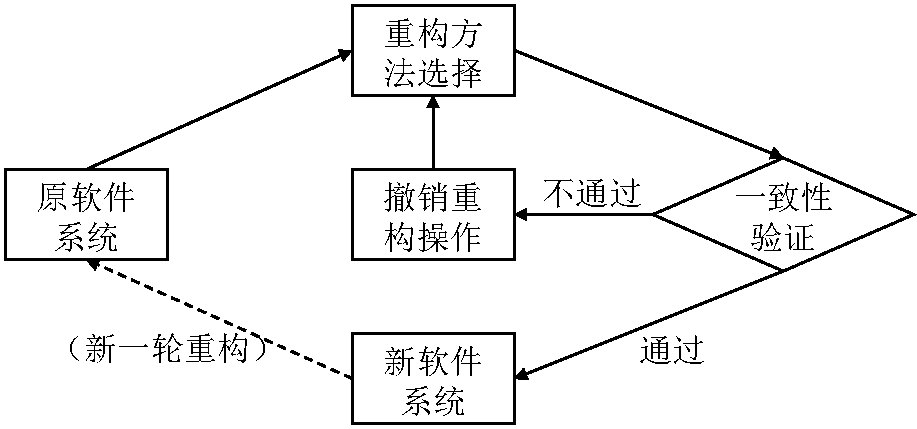
\includegraphics[height=45mm, width=90mm]{refactory.pdf}  
  \caption{\label{fig:refactory}软件重构一般过程}
\end{figure}

软件重构的一般是通过迭代转换的方式对软件系统进行转换。图~\ref{fig:refactory}描述了这样的转换过程。针
对原软件系统,每一轮迭代是对软件的一次小规模转换,针对特定代码选择某种重构方法,在实施软件重构操作后
测试其正确性,即测试软件的语义和功能是否与原来的保持一致。若测试通过,则本轮重构完成,软件维护人员可
在新的软件系统上进行新一轮重构。在任何时间一旦测试不通过,则最后一次程序转换撤销,需要重新选择重构方
法,换一种方式进行重构。通过很多轮这样的小规模程序转换,软件重构的过程和细节可以完全被软件维护人员所
掌控,并达到其所预想的效果。这样的迭代过程要求测试过程十分迅速,否则软件维护人员将不得不花费大量的时
间等待测试完成。因此,很多极限编程和其它敏捷软件开发的使用者将这种迭代过程作为软件开发周期的一个重要
组成部分。除此以外,为了减少一致性验证所带来的测试时间成本,部分学者提出使用先置性条件过滤,使得满足
条件的软件重构能保持语义和功能的一致性,从而减少不必要的测试成本。

研究者们提出了很多面向软件重构的技术和工具,主要分为两类:手动和自动化的方法。第一类方法主要通过开发
工具来为特定类型的手动重构操作提供技术支持~\cite{fowler1999refactoring, murphy2012we}。很多编辑器和
集成开发环境(IDE)中集成了这类重构支持工具,其作用仅仅是替软件维护人员执行指定的重构操作。这类方法
依赖于软件维护人员来识别某种重构类型适用于某处代码。因此,手动重构的过程较为复杂和乏味,软件维护人员
需要花费大量的时间和精力去识别重构机会。第二类方法通过自动推荐可以被开发人员采用的重构序列来提高软件
质量\cite{harman2007pareto, kessentini2011design, ouni2013maintainability, Silva2014}。这种序列可以
是一个完整的重构方案,即开发人员必须接受完整的解决方案;也可以是针对特定重构类型的推荐序列,开发人员
可以通过逐步交互的方法来完全控制他们所要应用的重构,通过有针对性的修复来提高软件质量。

大量的实践和研究表明,软件重构的作用主要有以下两种:(1)提高软件可维护性。当软件容易被理解时,软
件中的错误更容易被发现和修复~\cite{martin2009clean}。软件重构通过改进软件设计、重命名等方式,使得软
件设计更简单灵活、层次结构更清晰、代码更易被理解,从而减少代码维护的成本。(2)提高软件可扩展性。在
软件生命周期中,新的需求被不断添加,使得代码的复杂度越来越高,代码结构逐渐偏离原来的设计,从而导致了
扩展软件的难度越来越大。软件重构增加了程序设计的灵活性,通过改进软件设计,使得软件具备高凝聚、低耦合
和复杂度低等特点,将复杂代码变简单,从而提高代码的可扩展性。

\subsection{代码坏味与软件重构操作}
软件重构的时机通常与软件系统质量有关。软件质量下降时,软件系统发出需要重构的信号。最常见的情况是当软
件维护人员修补错误或添加新功能时,首先要需要做的就是理解代码。当代码可读性强,容易被理解时,修复软件
错误和添加新功能的效率更高。相反,当代码复杂度高、不容易被理解时,代码的质量下降,可维护性也随之降
低,此时通常需要对软件进行重构。重构软件可以加速当前和未来对代码的理解,从而提高软件维护效率。

代码坏味是软件系统中出现``坏代码''的信号,通常被研究者认为软件系统需要进行重构的信号。Fowler等人提出
了22种软件结构作为代码坏味,并认为这些代码坏味可以帮助软件维护人员决定软件是否需要被重构
~\cite{fowler1999refactoring}。针对这些代码坏味,Fowler等人提出了72代码重构操作,在保持程序外在行为
的一致性的同时,改进程序内部的设计结构~\cite{fowler1999refactoring}。在表~\ref{fig:badsmell}中我们列
举了其中十种较为经典的代码坏味,以及可能解决这些代码坏味的软件重构操作。

\begin{center}
\tablecaption{10中经典代码坏味}\label{fig:badsmell}
\begin{tabular}{|l|l|l|l|}
\hline
序号 & 代码坏味 & 软件重构操作 & 重构目标\\ \hline
1 & 代码重复 & 函数提炼、类提炼 & 提取公共代码\\ \hline
2 & 函数过长 & 函数提炼 & 拆分函数\\ \hline
3 & 类过大 & 类提炼 & 拆分类\\ \hline
4 & 参数过多 & 引入参数对象、函数替代参数 & 减少参数\\ \hline
5 & 发散式变化& 类提炼 & 将全部变化提取到新类\\ \hline
6 & 霰弹式改动& 函数移动、类内联 & 将全部修改合并为同类\\ \hline
7 & 依恋情节& 函数提炼、函数移动 & 移动依恋代码\\ \hline
8 & 数据泥团& 类提炼、引入参数对象 & 简化代码\\ \hline
9 & 基本类型偏执& 对象替换数据 & 简化代码 \\ \hline
10 & Switch语句 & 函数提炼、函数移动 & 减少Switch语句\\ \hline
\end{tabular}
\end{center}

代码坏味不是相互独立的,有一些代码坏味是相关联的,因此可以被相同的软件重构操作所解决。

有一些代码坏味是互斥的,因此它们所对应的软件重构操作也是相反的。

代码坏味是软件重构的重要信号,然而,软件重构却不完全是为了解决代码坏味。


\section{软件重构方法研究现状}
\subsection{软件重构检测}
\subsection{软件重构机会推荐}
\subsection{软件重构顺序推荐}
\subsection{软件重构一致性验证}

\section{本文的主要工作与创新点}

\section{论文的结构安排}

本模板参照南开大学学位论文写作规范编写,
仅仅提供了论文的基本格式,包括章节标题和正文字体、字号等等的设置。



您自愿使用这个模板。
提供本模板的目的是为了给您的论文写作带来方便,然而,
作者不保证这个模板完全符合学校的要求,也不对由此产生的任何后果负责。
如果您不同意这些条款,请不要使用这个模板。


\section{常用内容}

\begin{itemize}
	\item 参考文献的录入请参考\ref{sec:relatedwork:ref};
	\item 图片插入参考\ref{sec:relatedwork:table};
	\item 分数和公式参考\ref{sec:relatedwork:equation};
	\item Latex绘图工具参考\ref{sec:method:tikz};
	\item 代码块参考\ref{sec:method:code};
\end{itemize}